\documentclass[12pt]{article}

\usepackage{graphicx}
\usepackage{fancyhdr}
\usepackage{biblatex}
\usepackage{rotating}
\usepackage{xcolor}
\usepackage{listings}
\usepackage{indentfirst}
\usepackage{float}
\usepackage{url}
\usepackage{longtable}
\usepackage[margin=1in]{geometry}

\bibliography{bib.bib}
\setlength{\parskip}{\baselineskip}%

\lstset{basicstyle=\ttfamily,
  showstringspaces=false,
  commentstyle=\color{red}
  keywordstyle=\color{blue}
}

\title{CS 751: Introduction to Digital Libraries - Assignment 3}
\author{Jessica McConnell}
\date{\today}

\begin{document}
\maketitle

\section{Q1}
For this question we had to set up boilerpipe and run our 10,000 body files we downloaded from assignment 1 through it to remove all html templates.

I used the boilerpipe application suggested in the Assignment 3 powerpoint by Christian Kohlschütter. \nocite{Kohlschütter:2011:boilerpipe}
\subsection{Picking Files}
I began by running through all the files I had downloaded. As a reminder from assignment 1, I only downloaded the final unique URIs after all redirects from the original 10000 unique URIs. This did not give me 10,000 final unique pages instead it was 7405 final unique pages. I also was unable to download 477 pages originally. In my testing I also learned that the boilerpipe method did not accept files that were .htm files so I threw those out.  I only ran the 6810 files that ended in .html boilerpipe.

\begin{lstlisting}[language=bash]
for line in `ls -d */`; do 
    item=$(ls $line); 
    if [[ -z "$item" ]]; then 
        echo $line "empty"; 
    elif [[ "$item" == *.html ]]; then 
        echo $line$item" Good"; 
    else echo $line$item" Bad"; 
    fi; 
done > files
\end{lstlisting}

\subsection{Running Files}
I wrote a java file to perform my boilerpipe tasks called `A3.java'.  It takes all the file names in the `GoodFiles' and runs the file through boilerpipe ArtifactExtract.  I compiled and ran my java file with the following 2 commands:

\begin{lstlisting}[language=bash]
javac -d . -cp .:./boilerpipe-1.2.0/boilerpipe-1.2.0.jar: - 
./boilerpipe-1.2.0/nekohtml-1.9.13.jar:./boilerpipe-1.2.0/ - 
xerces-2.4.0.jar:./boilerpipe-1.2.0/* A3.java

java -cp .:./boilerpipe-1.2.0/boilerpipe-1.2.0.jar: - 
./boilerpipe-1.2.0/nekohtml-1.9.13.jar:./boilerpipe - 
-1.2.0/xerces-2.4.0.jar:./boilerpipe-1.2.0/* A3
\end{lstlisting}

I received exceptions on four files.  Three of the files had a non-english character in the name and the java application could not find it.  I am not sure why it could not find the fourth file though.  However, I also could not cat the file directly.  There must be something wrong with the file for the fourth exception received. The exceptions are below.

\begin{lstlisting}[language=Java]
Exception in thread "main" java.io.FileNotFoundException: -
../bodies/328/mushroom-networks-adds-voip-armor� - 
%84�-its-truffle-broadband-bonding�%84�-network-appliance.html 
(No such file or directory)
        at java.io.FileInputStream.open(Native Method)
        at java.io.FileInputStream.<init>(FileInputStream.java:146)
        at java.io.FileInputStream.<init>(FileInputStream.java:101)
        at java.io.FileReader.<init>(FileReader.java:58)
        at A3.main(A3.java:36)


Exception in thread "main" java.io.FileNotFoundException: -
../bodies/5805/saddle-�%80%94-markens-charles.html -
(No such file or directory)
        at java.io.FileInputStream.open(Native Method)
        at java.io.FileInputStream.<init>(FileInputStream.java:146)
        at java.io.FileInputStream.<init>(FileInputStream.java:101)
        at java.io.FileReader.<init>(FileReader.java:58)
        at A3.main(A3.java:36)

Exception in thread "main" java.io.FileNotFoundException: -
../bodies/6262/what-do-you-mean-there�%80%99s-child-slave -
-labor-my-chocolate.html (No such file or directory)
        at java.io.FileInputStream.open(Native Method)
        at java.io.FileInputStream.<init>(FileInputStream.java:146)
        at java.io.FileInputStream.<init>(FileInputStream.java:101)
        at java.io.FileReader.<init>(FileReader.java:58)
        at A3.main(A3.java:36)

Exception in thread "main" java.io.FileNotFoundException: -
m./bodies/999/index.html?utm_source=twitterfeed&utm_medium= -
twitter.html (No such file or directory)
        at java.io.FileInputStream.open(Native Method)
        at java.io.FileInputStream.<init>(FileInputStream.java:146)
        at java.io.FileInputStream.<init>(FileInputStream.java:101)
        at java.io.FileReader.<init>(FileReader.java:58)
        at A3.main(A3.java:36)
\end{lstlisting}

\begin{lstlisting}[language=bash]
jmcconne@sirius:~/cs751/a3$ ls ../bodies/999/
index.html?utm_source=twitterfeed&utm_medium=twitter.html
jmcconne@sirius:~/cs751/a3$ cat ../bodies/999/index.html? -
    utm_source=twitterfeed&utm_medium=twitter.html
cat: ../bodies/999/index.html?utm_source=twitterfeed: -
    No such file or directory
\end{lstlisting}

\subsection{Unsuccessful Documents After Boilerpipe}
After running boilerpipe, I had 329 files that returned with no size. Doing a random sampling of the empty files they appear to consist of blogs that only contain photos, iTunes pages, only pictures and sites that used a smaller URI that translated to a longer URI. For example \url{smarturl.it} links.

A few of the links it was unsuccessful for:\\
Pictures only:\\
\url{http://rcobanus.dailyfunnypics.me/young-boy-returns-home-with-a-new-porsche-this-is-priceless}
\url{http://newzcard.com/card/mBN5VP/singers-usher-l-and-rihanna-arrive-at-the-2010-american-music-awards-held-at-nokia-theatre-l-a-live(mBN5VP)?r=UsherPics}

Shortened URLs:\\
\url{http://smarturl.it/FourFiveSeconds}
\url{http://smarturl.it/NBBiTunesDLX}
\url{http://nblo.gs/133ljo}

For my sampling of unsuccessful pages, the original sizes for the html download varied between 2000 and 6000 bytes. The HTML web pages also varied from 50 unique words to approximately 250 unique words.

\subsection{Successful Documents After Boilerpipe}
For my sampling of successful web pages they included:\\
1. a login page for the New York Times \url{https://myaccount.nytimes.com/auth/login?URI=http%3A%2F%2Fwell.blogs.nytimes.com%2F2015%2F01%2F06%2Fjunk-food-in-the-new-year%2F%3Fpartner%3Drss%26emc%3Drss%26utm_content%3Dbuffera524f%26utm_medium%3Dsocial%26utm_source%3Dtwitter.com%26utm_campaign%3Dbuffer%26_r%3D5&REFUSE_COOKIE_ERROR=SHOW_ERROR}\\
2. a Twitter post \url{https://twitter.com/BernieceBryon/status/561189374608420864}\\
3. a website about a festival that uses a very common page layout \url{http://www.usafestival.net/?page=details&id=7117}\\
4. an article from the huffingtonpost \url{http://www.huffingtonpost.com/2015/01/30/super-bowl-trivia_n_6543044.html?utm_hp_ref=religion&ir=Religion&utm_medium=twitter&utm_source=twitterfeed}

The sizes of the web pages that were successful was much larger than the unsuccessful pages with a range from 30,000 bytes to 330,000 bytes.  The unique words before boiler pipe was applied ranged from 600 to just over 9000 words. After boiler pipe was applied the unique words ranged from 20 to 8000 words. This change is indicative of websites that use common html website layouts that the boilerpipe tool can easily identify. The is easily expected just by looking at the random sample of URIs I used for my successful documents. Three out of the four documents originated from very popular websites with a defined layout that includes changing content and not just pictures.

\section{Q2}
For this question we were to get all unique words from the files before and after boilerpipe was applied. We had to graph the word rank vs word frequency and compare it to a Zipf distribution. We also had to apply a stop word list to the most common words.

\subsection{Getting the Unique Words}
I wrote two python scripts to get the unique words and count for me.  They are called `textStats.py' and `bodyStats.py'.  They essentially performed the same actions with some brief differences in how the files were found and some of the exceptions.  To try to get the most accurate unique word assessment I removed all colons, question marks, exclamation points, commas and periods from the ends of words.  I also took out all new lines and tabs.  Specifically for the html documents I also removed curly brackets, single character words that were not letters, slashes and arrows.  I used the python Counter function to get my word rank.

TEXT COMMAND:\\
\begin{lstlisting}[language=bash]
    python ./textStats.py ./bodyFiles/
\end{lstlisting}

HTML COMMAND:\\
\begin{lstlisting}[language=bash]
    python ./bodyStats.py ./GoodFiles
\end{lstlisting}


\begin{longtable}{|c|c|c|c|}
    \hline
    \multicolumn{2}{|c}{HTML} & \multicolumn{2}{|c|}{Text}\\
    \hline
    Word & Count & Word & Count \\
    \hline
    \endfirsthead
    \multicolumn{4}{c}{Continued from previous page}\\
    \hline
    \multicolumn{2}{|c}{HTML} & \multicolumn{2}{|c|}{Text}\\
    \hline
    Word & Count & Word & Count \\
    \hline
    \endhead
    div & 2278100 & the & 91917 \\
    \hline
    a & 1771169 & to & 50881 \\
    \hline
    span & 1274771 & and & 50490 \\
    \hline
    li & 910908 & of & 42374 \\
    \hline
    script & 312721 & a & 41382 \\
    \hline
    the & 286658 & in & 31828 \\
    \hline
    td & 285403 & is & 21936 \\
    \hline
    p & 254866 & for & 21330 \\
    \hline
    to & 222278 & you & 17413 \\
    \hline
    and & 189165 & on & 16823 \\
    \hline
    ul & 185602 & that & 16523 \\
    \hline
    img & 183164 & this & 13324 \\
    \hline
    tr & 174607 & with & 12768 \\
    \hline
    meta & 167120 & it & 12479 \\
    \hline
    of & 147523 & or & 11440 \\
    \hline
    i & 141436 & your & 10538 \\
    \hline
    in & 141426 & are & 10212 \\
    \hline
    option & 127241 & be & 10168 \\
    \hline
    button & 105802 & as & 9749 \\
    \hline
    for & 104511 & at & 9711 \\
    \hline
    h3 & 104190 & i & 9430 \\
    \hline
    var & 99351 & by & 8798 \\
    \hline
    b & 95416 & have & 8094 \\
    \hline
    false & 90511 & from & 7598 \\
    \hline
    br & 90297 & was & 7574 \\
    \hline
    link & 88180 & not & 7165 \\
    \hline
    type="text/javascript" & 82765 & an & 7012 \\
    \hline
    on & 82258 & will & 6954 \\
    \hline
    input & 79806 & we & 6809 \\
    \hline
    table & 74401 & new & 5854 \\
    \hline
    is & 74079 & if & 5531 \\
    \hline
    this & 72885 & but & 5485 \\
    \hline
    your & 70506 & more & 5334 \\
    \hline
    you & 69909 & has & 5333 \\
    \hline
    if & 64528 & can & 5179 \\
    \hline
    with & 61316 & all & 5076 \\
    \hline
    target="\_blank" & 60132 & they & 4815 \\
    \hline
    new & 57480 & about & 4431 \\
    \hline
    h2 & 55091 & shipping & 4409 \\
    \hline
    null & 52895 & one & 4398 \\
    \hline
    by & 50978 & their & 4199 \\
    \hline
    strong & 48891 & out & 4173 \\
    \hline
    label & 48097 & he & 4082 \\
    \hline
    it & 47847 & our & 4059 \\
    \hline
    type="button" & 43248 & get & 4037 \\
    \hline
    or & 42528 & time & 4003 \\
    \hline
    all & 41396 & other & 3946 \\
    \hline
    function & 39852 & when & 3907 \\
    \hline
    rel="nofollow" & 39702 & my & 3659 \\
    \hline
    that & 38959 & up & 3649 \\
    \hline
\end{longtable}

\subsection{Stop Words}

I chose to use the stopwords list that is a Default English stopwords list. I found the list at Ranks NL \nocite{Doyle:ranksNL}.  Below are the words in the list.

\begin{longtable}{|c|c|c|c|c|}
    \hline
    \multicolumn{5}{|c|}{Stop Words} \\
    \hline
    \endfirsthead
    \multicolumn{5}{c}{Continued from previous page}\\
    \hline
    \multicolumn{5}{|c|}{Stop Words} \\
    \hline
    \endhead
    a & don't & in & she'll & we\\
    \hline
    about & down & into & she's & we'd\\
    \hline
    above & during & is & should & we'll\\
    \hline
    after & each & isn't & shouldn't & we're\\
    \hline
    again & few & it & so & we've\\
    \hline
    against & for & it's & some & were\\
    \hline
    all & from & its & such & weren't\\
    \hline
    am & further & itself & than & what\\
    \hline
    an & had & let's & that & what's\\
    \hline
    and & hadn't & me & that's & when\\
    \hline
    any & has & more & the & when's\\
    \hline
    are & hasn't & most & their & where\\
    \hline
    aren't & have & mustn't & theirs & where's\\
    \hline
    as & haven't & my & them & which\\
    \hline
    at & having & myself & themselves & while\\
    \hline
    be & he & no & then & who\\
    \hline
    because & he'd & nor & there & who's\\
    \hline
    been & he'll & not & there's & whom\\
    \hline
    before & he's & of & these & why\\
    \hline
    being & her & off & they & why's\\
    \hline
    below & here & on & they'd & with\\
    \hline
    between & here's & once & they'll & won't\\
    \hline
    both & hers & only & they're & would\\
    \hline
    but & herself & or & they've & wouldn't\\
    \hline
    by & him & other & this & you\\
    \hline
    can't & himself & ought & those & you'd\\
    \hline
    cannot & his & our & through & you'll\\
    \hline
    could & how & ours    ourselves & to & you're\\
    \hline
    couldn't & how's & out & too & you've\\
    \hline
    did & i & over & under & your\\
    \hline
    didn't & i'd & own & until & yours\\
    \hline
    do & i'll & same & up & yourself\\
    \hline
    does & i'm & shan't & very & yourselves\\
    \hline
    doesn't & i've & she & was & \\
    \hline
    doing & if & she'd & wasn't & \\
    \hline
\end{longtable}

I created a python script named `wordCompare.py' to perform the comparisons between the two lists. I used the commands below to get my results.

HTML:\\
\begin{lstlisting}[language=bash]
    python wordCompare.py htmlFilesWords stoplist
\end{lstlisting}

Text: \\
\begin{lstlisting}[language=bash]
    python wordCompare.py textFilesWords stoplist
\end{lstlisting}

From the Text list there were 43 words in the stop list.  In the HTML list there were only 20 words in the stop list.  The words remaining in each list can be seen in the table below.
\begin{longtable}{|c|c|}
    \hline
    \multicolumn{2}{|c|}{After Stop Words}\\
    \hline
    Text & HTML \\
    \hline
    \endfirsthead
    \multicolumn{2}{c}{Continued from previous page}\\
    \hline
    \multicolumn{2}{|c|}{After Stop Words}\\
    \hline
    Text & HTML \\
    \hline
    \endhead
    will & div\\
    \hline
    new & span\\
    \hline
    can & li\\
    \hline
    shipping & script\\
    \hline
    one & td\\
    \hline
    get & p\\
    \hline
    time & ul\\
    \hline
    & img\\
    \hline
    & tr\\
    \hline
    & meta\\
    \hline
    & option\\
    \hline
    & button\\
    \hline
    & h3\\
    \hline
    & var\\
    \hline
    & b\\
    \hline
    & br\\
    \hline
    & link\\
    \hline
    & type="text/javascript"\\
    \hline
    & input\\
    \hline
    & table\\
    \hline
    & target="\_blank"\\
    \hline
    & new\\
    \hline
    & h2\\
    \hline
    & null\\
    \hline
    & strong\\
    \hline
    & label\\
    \hline
    & false\\
    \hline
    & type="button"\\
    \hline
    & function\\
    \hline
    & rel="nofollow"\\
    \hline
\end{longtable}

\subsection{Graphs}
Both graphs follow a zipf distribution.  A zipf distribution has some very popular items followed by a much larger popularion of less popular items.  The graph looks similar to a reverse log graph.

\begin{figure}[H]
    \centering
    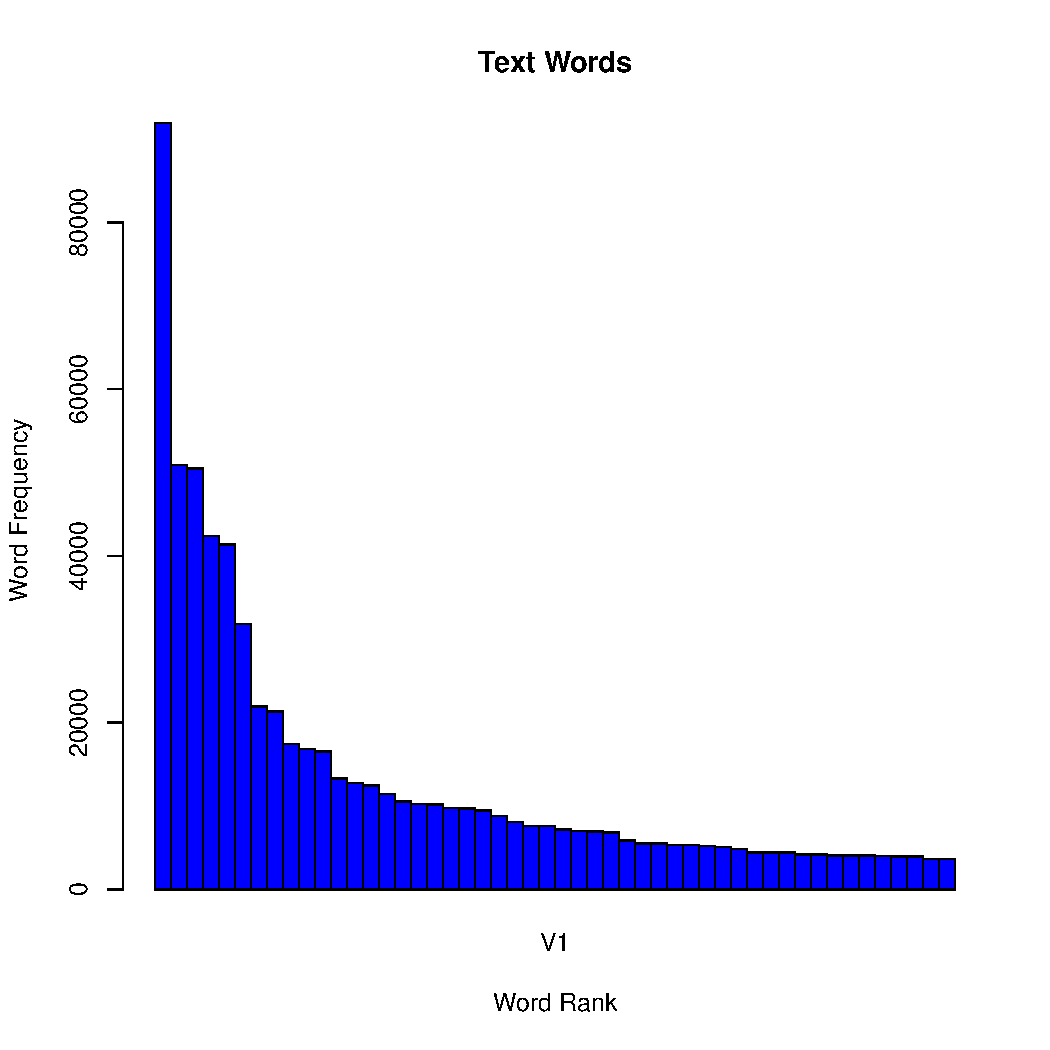
\includegraphics[scale=0.7]{text.pdf}
\end{figure}

\begin{figure}[H]
    \centering
    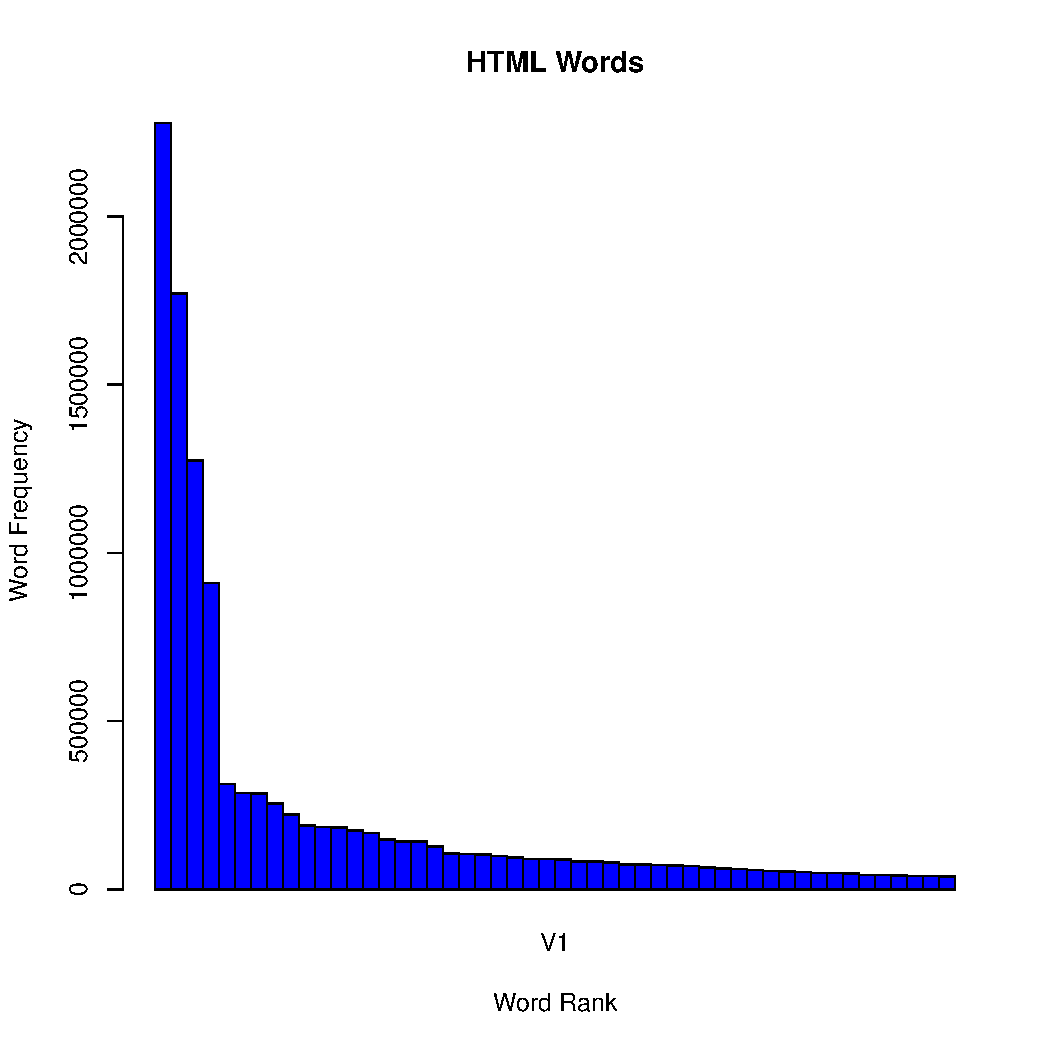
\includegraphics[scale=0.7]{html.pdf}
\end{figure}

\printbibliography

\end{document}
